\documentclass{article}

\usepackage[left=1.25in,top=1.25in,right=1.25in,bottom=1.25in,head=1.25in]{geometry}
\usepackage{amsfonts,amsmath,amssymb,amsthm}
\usepackage{verbatim,float,url,enumerate}
\usepackage{graphicx,subfigure,psfrag}
\usepackage{natbib}
\usepackage{environ}
\usepackage{hyperref}
\usepackage{pifont}
\usepackage{xcolor}

\newtheorem{algorithm}{Algorithm}
\newtheorem{theorem}{Theorem}
\newtheorem{lemma}{Lemma}
\newtheorem{corollary}{Corollary}

\theoremstyle{remark}
\newtheorem{remark}{Remark}
\theoremstyle{definition}
\newtheorem{definition}{Definition}

\newcommand{\argmin}{\mathop{\mathrm{argmin}}}
\newcommand{\argmax}{\mathop{\mathrm{argmax}}}
\newcommand{\minimize}{\mathop{\mathrm{minimize}}}
\newcommand{\maximize}{\mathop{\mathrm{maximize}}}
\newcommand{\st}{\mathop{\mathrm{subject\,\,to}}}
\newcommand{\dist}{\mathop{\mathrm{dist}}}

\newcommand{\reals}{\mathbb R}
\newcommand{\prox}{\operatorname{prox}}
\newcommand{\dom}{\operatorname{dom}}
\def\R{\mathbb{R}}
\def\E{\mathbb{E}}
\def\P{\mathbb{P}}
\def\Cov{\mathrm{Cov}}
\def\Var{\mathrm{Var}}
\def\half{\frac{1}{2}}
\def\sign{\mathrm{sign}}
\def\supp{\mathrm{supp}}
\def\th{\mathrm{th}}
\def\tr{\mathrm{tr}}
\def\dim{\mathrm{dim}}
\def\hbeta{\hat{\beta}}

\begin{document}

\title{Bicycle Model}
\author{\Large Josh Bennett, jjbennet@andrew.cmu.edu}
\maketitle

\section{Derivation}

\begin{figure}[H]
    \label{fig:bicycle_model}
    \centering
        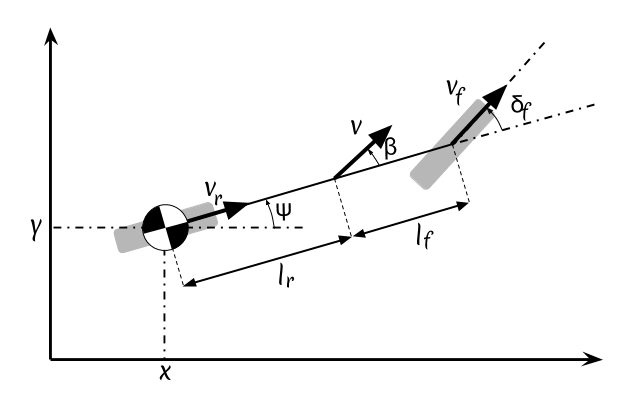
\includegraphics[width=0.95\textwidth]{bicycle_model_diagram.png}
    \caption{Bicycle model state variable diagram.}
\end{figure}

Some preliminary relationships:

State variables:

$$ z = \left \lbrack \begin{array}{c}  x \\ y \\ \psi \\ \delta_f \\ v_f \end{array} \right \rbrack $$

We will use $v_f$ as the state variable for velocity to avoid discontinuities.

$$ v_r = v_f \cos {( \delta_f) } $$
$$ \dot{\psi} = v_f \sin {( \delta_f) } $$

We will assume a front wheel drive vehicle with wheel torque $\tau$ and wheel radius $r$, generating a force of $\frac{\tau} r$ as an input. Assuming a mass $m$ and an inertia $I$ for the vehicle defined as the inertia at the wheel base, not the center of mass, we can derive the following equation for the acceleration of the front wheel:

$$ a_f = \frac{\tau}{r} \left ( \frac {1} {m \cos {( \delta_f) }} + \frac {\left((l_r+l_f\right)\sin {( \delta_f) } )^2} {I} \right ) $$

We will also assume that the steering angle is controlled by some steering rate input $w$

$$ \left \lbrack \arraycolsep=1.4pt\def\arraystretch{1.5} \begin{array}{c}
    \dot{x} \\
    \dot{y} \\
    \dot{\psi} \\
    \dot{\delta_f} \\
    \dot{v_f}
\end{array} \right \rbrack  = \left \lbrack \arraycolsep=1.4pt\def\arraystretch{1.5} \begin{array}{c}
    v_f \cos {( \delta_f) } \cos{( \psi )} \\
    v_f \cos {( \delta_f) } \sin{( \psi )} \\
    \frac {v_f \sin {( \delta_f) }} {l_r + l_f} \\
    0 \\
    0
\end{array} \right \rbrack + \left \lbrack \arraycolsep=1.4pt\def\arraystretch{1.5} \begin{array}{c}
    0 \\
    0 \\
    0 \\
    w \\
    a_f
\end{array} \right \rbrack $$

\end{document}
